\let\negmedspace\undefined
\let\negthickspace\undefined
\let\vec\mathbf
\newcommand{\myvec}[1]{\ensuremath{\begin{pmatrix}#1\end{pmatrix}}}
\documentclass[journal,12pt,twocolumn]{IEEEtran}
\usepackage{gensymb}
\usepackage{amssymb}
\usepackage[cmex10]{amsmath}
\usepackage{amsthm}
\usepackage[export]{adjustbox}
\usepackage{bm}
\usepackage{float}
\usepackage{caption}
\usepackage{longtable}
\usepackage{enumitem}
\usepackage{mathtools}
 \usepackage{tikz}
\usepackage[breaklinks=true]{hyperref}
\usepackage{listings}
\usepackage{color}                                            %%
\usepackage{array}                                            %%
\usepackage{longtable}                                        %%
\usepackage{calc}                                             %%
\usepackage{multirow}                                         %%
\usepackage{hhline}                                           %%
\usepackage{ifthen}                                           %%
\usepackage{lscape}     
\usepackage{multicol}
% \usepackage{enumerate}
\DeclareMathOperator*{\Res}{Res}
\renewcommand\thesection{\arabic{section}}
\renewcommand\thesubsection{\thesection.\arabic{subsection}}
\renewcommand\thesubsubsection{\thesubsection.\arabic{subsubsection}}
\renewcommand\thesectiondis{\arabic{section}}
\renewcommand\thesubsectiondis{\thesectiondis.\arabic{subsection}}
\renewcommand\thesubsubsectiondis{\thesubsectiondis.\arabic{subsubsection}}
\hyphenation{op-tical net-works semi-conduc-tor}
\def\inputGnumericTable{}                                 %%
\lstset{
frame=single, 
breaklines=true,
columns=fullflexible
}
\begin{document}

\raggedbottom
\setlength{\parindent}{0pt}
\vspace{3cm}
\title{AI1110 - Assignment 2}
\author{Vedant Bhandare\\CS21BTECH11007}
\maketitle
\newpage
\bigskip
\renewcommand{\thefigure}{\theenumi}
\renewcommand{\thetable}{\theenumi}
\maketitle

Download all python codes from 
\begin{lstlisting}
https://github.com/TYCN129/AI1110-Assignments/tree/main/Assignment%202/Codes
\end{lstlisting}
%
and latex codes from 
%
\begin{lstlisting}
https://github.com/TYCN129/AI1110-Assignments/tree/main/Assignment%202
\end{lstlisting}
\textbf{ICSE class 12 - 2019 paper}

\section{\textbf{QUESTION - 18}}
Draw a sketch and find the area bounded by the curve $x^2 = y$ and $x + y = 2$
\section{\textbf{SOLUTION}}
We have the curves
\begin{align}
    x + y &= 2\\
    x^2 &= y
\end{align}
We can observe that the point $(1,1)$ passes through the line. Let this point be called P. The line could be represented as,\\
\begin{align}
    \vec{X} &= P + \lambda \vec{m}\\
    \vec{X} &= \myvec{1 \\ 1} + \lambda \myvec{1 \\ m}
\end{align}
where m is slope of the line and is equal to -1
\begin{align}
    \vec{X} &= \myvec{1 + \lambda \\ 1 + \lambda m}\\
    \vec{X} &= \myvec{1 + \lambda \\ 1 - \lambda}
\end{align}
Also the equation for parabola in vector form is,
\begin{align}
    \vec{X}^{\top}A\vec{X} + B^{\top}\vec{X} + C = 0
\end{align}
For the parabola $x^2 - y = 0$, $A = \myvec{1 & 0 \\ 0 & 0}$,\\ $B = \myvec{0 \\ -1}$ and $C$ is null matrix
Thus,
\begin{align}
    \vec{X}^{\top} \myvec{1 & 0 \\ 0 & 0}\vec{X} + \myvec{0 & -1}\vec{X} = 0
\end{align}
Substituting equation (6) in equation (8), we get
\begin{align}
    \myvec{1 + \lambda & 1 - \lambda}\myvec{1 & 0 \\ 0 & 0}\myvec{1 + \lambda \\ 1 - \lambda} + \\ \myvec{0 & -1}\myvec{1 + \lambda \\ 1 - \lambda} = 0\\
    (1 + \lambda)^2 - (1 - \lambda) = 0\\
    \lambda^2 + 3\lambda = 0
\end{align}
Equation (12) is quadratic and of the form $ax^2 + bx + c = 0$, where $a = 1, b = 3$ and $c = 0$\\
Using the quadratic formula
\begin{align}
    x &= \frac{-b \pm \sqrt{b^2 - 4ac}}{2a}\\
    \lambda &= \frac{-3 \pm \sqrt{3^2 - 4(1)(0))}}{2(1)}\\
    \lambda &= \frac{-3 + 3}{2}, \frac{-3 - 3}{2}\\
    \lambda &= 0, -3
\end{align}
On substituting the values of $\lambda$ in equation (6), we get the points of intersection,
\begin{align}
    \vec{X_1}^{\top} &= \myvec{1 \\ 1}\\
    \vec{X_2}^{\top} &= \myvec{-2 \\ 4}
\end{align}
Thus, the two curves intersect at the points (-2 , 4) and (1 , 1)

\clearpage

\begin{figure}[t]
    \centering
    \includegraphics[width=\columnwidth]{Question.png}
    \caption*{Fig 1: Graph Plot}
    \label{fig:graph}
\end{figure}

\subsection{\textbf{Area of trapezium ABCD (A_1)}}
\begin{figure}[h]
    \centering
    \includegraphics[width=\columnwidth]{trapezium.png}
    \caption*{Fig 3: Trapezium ABCD}
    \label{fig:trap}
\end{figure}
\begin{align}
    A_1 &= \frac{1}{2}\times(AB + CD)\times AD\\
    A_1 &= \frac{1}{2}\times(4 + 1)\times 3
\end{align}
\begin{center}
    \fbox{A_1 = 7.5 sq.units}
\end{center}
\subsection{\textbf{Area under the curve $x^2 = y$ (A_2)}}
\begin{figure}[H]
    \centering
    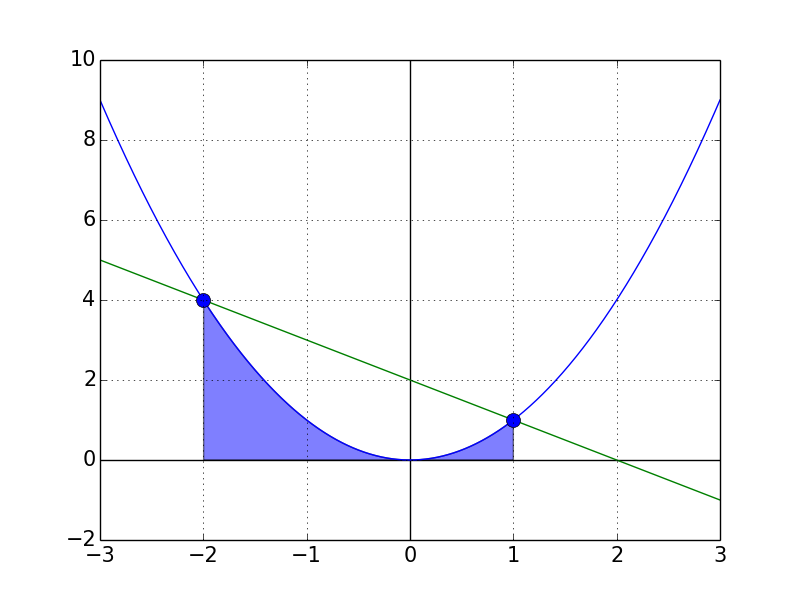
\includegraphics[width=\columnwidth]{x^2.png}
    \caption*{Fig 4: Region below curve $x^2 = y$}
    \label{fig:x^2}
\end{figure}
\begin{align}
    A_2 &= \int_{-2}^{1} x^2 \, dx\\
    A_2 &= \frac{x^3}{3}\Biggr|_{-2}^{1}\\
    A_2 &= \frac{(1)^3}{3} - \frac{(-2)^3}{3}
\end{align}
\begin{center}
    \fbox{A_2 = 3 sq.units}
\end{center}    
\subsection{\textbf{Area of the shaded region}}
\begin{align}
    A &= A_1 - A_2\\
    A &= 7.5 - 3\\
\end{align}
\begin{center}
    \textbf{\fbox{A = 4.5 sq.units}}
\end{center}
\begin{figure}[H]
    \centering
    \includegraphics[width=\columnwidth]{Sketch.png}
\end{figure}
\begin{center}
\textbf{The area bound by the curves $x^2 = y$ and $x + y = 2$ is 4.5 sq.units}
\end{center}
\end{document}
